%!TeX root=Main Document/Dissertation.tex

\section{Methodology}
An application was produced to test the hypothesis. This application used the Games Education Framework (GEF) [reference] as the framework, which was chosen based on its lightweight overhead, its portability and recommendations from several university lecturers. It was developed using Visual Studio 2017 in C++, both tools chosen due to the author's familiarity with them and the flexibility afforded by both.

GitHub Desktop was used as the tool for source control, ensuring risks to the project were kept to a minimum. Further to this, a GitFlow tool was developed in order to stem the risk of pushing and pulling work from incorrect branches, and prevent any conflicts when committing and pushing new work.

\subsection{Application Design}
The application was designed through an iterative process. 

\begin{figure}
	%\includegraphics[width=\linewidth]{../Images/ClassDiagram.png}
	\caption{A UML Class Diagram of the Application}
	\label{fig:classdiagram}
\end{figure}

\subsection{Test Environment Design}
The application simulated an environment, in which two flocks interact (one of which is improved via a genetic algorithm) within a limited space of scarce resources, with the aim of finding out if a flocking algorithm improved by a genetic algorithm can out-compete one without.

To answer the research question required removing as many base assumptions as possible - reducing the problem to its core necessities. To do that, three core decisions were made: The environment should be limited so as to keep the flocks in competition with each other, this means the flocks have to interact; there should be a limited amount of resources in the environment, less than that required to support two full populations of flocks, this should drive the flocks to compete over resources spawned in the environment; finally there should only be two flocks, one improved by a genetic algorithm over simulated generations and one produced through a tested expanded flocking algorithm design. This ensures a competitive environment in which the effects of decisions the genetic algorithm makes can be singled out, and the data produced analysed. Fig.\ref{fig:EnvScrnshot} displays a screenshot of this environment in action.
\begin{figure}
	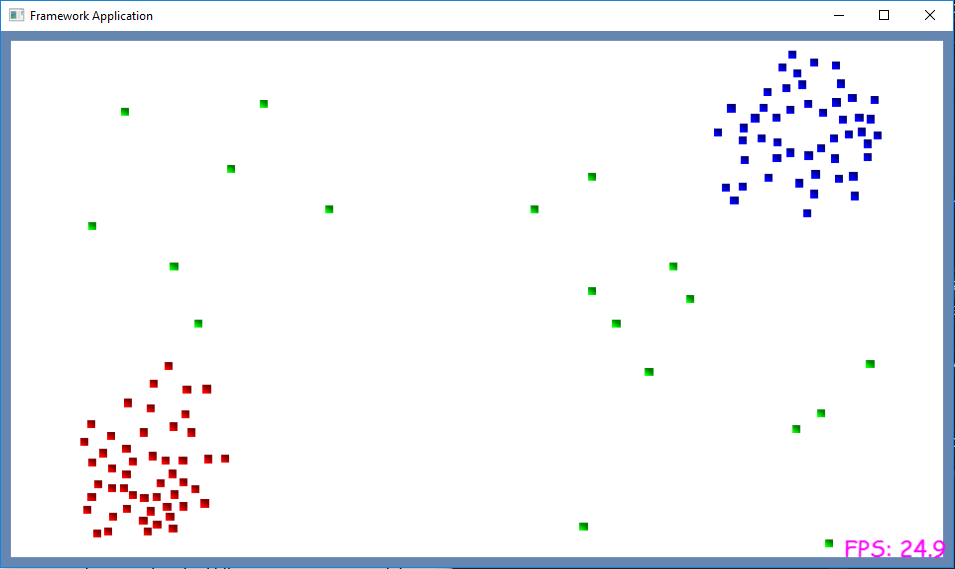
\includegraphics[width=\linewidth]{../Images/EnvironmentScreenshot.png}
	\caption{A screenshot of the test environment in action: in red the regular flock; in blue the genetic algorithm modified flock; in green resources. The white area indicates the space in which the boids can move}
	\label{fig:EnvScrnshot}
\end{figure}


\subsection{Flocking Algorithm Design}
The flocking algorithm was originally designed primarily by adapting the example from \citet{flockingprocessingorg}. As this was a very clear representation of how to design a basic flocking algorithm from a code perspective. There were also clear areas for improving the efficiency of the algorithm presented too. The most major way was combining the calculations for Alignment, Separation and Cohesion. This was so each boid was not checking against all others for each force calculation, and only needed to check against all other boids once instead of three times; doing that was simple and reduced the requirement for N-Body problem solutions like the Barnes-Hut algorithm later on. The other main way was combining the calculations required for each force as they use shared variables, so calculating them once instead of multiple times for each force also increased efficiency.

This worked ok for the original three forces based on \citet{Reynolds:1987:FHS:37402.37406}. However, issues came up when expanding the application to include extra forces. Especially since in the aforementioned implementation it wasn't strictly clear how the forces would graph out due to the lack of separation between direction and weighting. This caused issues to pile up and it was clear a change in the flocking algorithm design was necessary to expand and edit the program appropriately.

The boids' forces as they are in the final program were modelled primarily off \citet{4604156}, which has a very clear mathematical representation of each force. The version of the expanded boids algorithm found in this paper was modified by optimising the algorithm for the environment in which it was placed. The forces each boid experienced were: Cohesion, Alignment, Separation, Food Attraction and Flock Avoidance. Each of these forces were the result of multiplication of a unit vector and their respective weight, mathematically represented in Eq.\ref{forcevector_equation}

\begin{equation}
\boldsymbol{Force Vector} = \boldsymbol{v} \cdot \boldsymbol{w}
\label{forcevector_equation}
\end{equation}
Where $\boldsymbol{v}$ is the unit vector which describes the direction of the force, and $\boldsymbol{w}$ is the weight that magnifies the force dependent on its relation to its environment.

The relationship of the weight to the unit vector will become clear as the boid forces are described further on. This separation of direction vector and weight, meant it was far easier to mathematically model and graph out each force to predict their behaviour; this caused a reduction to the amount of work necessary to produce a functioning flocking algorithm. The resulting accelerative force then is the sum of these forces. That sum is then used in the Semi-Implicit Euler method to produce the updated position of each boid every frame.

\subsubsection{Cohesion} 
This is the first of the boid forces, cohesion pulls the boid in the direction of flock members, in this case towards its local flock centre. The boids local flock centre is determined by its neighbours in communicable range and is the average position of those flock members. The further the distance away from its neighbours, the stronger the force. Below is Eq.\ref{cohesion_equation} describing the direction vector and weighting:
\begin{equation}
\begin{split}
	\boldsymbol{\hat{v}_{coh}} &= \frac{ LFCVector} {|LFCVector|} \\
	\boldsymbol{w_{coh}} &= \frac{(|LFCPos - BoidPos|)^2} {30 \cdot FlockSize}
\end{split}
\label{cohesion_equation}
\end{equation}
Where $LFCVector$ represents the vector from the boid to the local flock centre, $LFCPos$ is the position of the local flock centre, $BoidPos$ is the position of the boid and $FlockSize$ is the number of flock members as a whole.

\subsubsection{Alignment}
Alignment is a vector that accelerates the boid in the average direction of its neighbouring boids. This produces the common direction the flock as the boids individually move about. By taking the average velocity of neighbouring boids as a direction vector and multiplying it one over the distance between the local flock centre and itself a suitable alignment vector is produced. Below is Eq.\ref{alignment_equation} describing the two components of the alignment vector:
\begin{equation}
\begin{split}
	\boldsymbol{\hat{v}_{ali}} &= \frac{ LFVelVector} {|LFVelVector|} \\
	\boldsymbol{w_{ali}} &= \frac{1} {10 \cdot |(LFCPos - BoidPos)|}
\end{split}
\label{alignment_equation}
\end{equation}
Where $LFVelVector$ is the average velocity of the local flock members, and $LFCPos$ and $BoidPos$ are the same as in Eq.\ref{cohesion_equation}.

\subsubsection{Separation}
Separation is the force that stops flocks getting too tightly knit. By having enough space between flock members it grants maneuverability where there would otherwise be collisions that slow movement down; that could be from obstacles, other moving entities or other boids in the flock. The unit vector that represents the direction for the force to be applied is calculated by taking the negative of the vector to the nearest neighbouring boid; multiplying that by the weighted multiple of the number of neighbours divided by the distance to the closest neighbour produces the separation vector described below in Eq.\ref{separation_equation}:
\begin{equation}
\begin{split}
	\boldsymbol{\hat{v}_{sep}} &= -\frac{ClosestNeighbourVector} {| ClosestNeighbourVector|} \\
	\boldsymbol{w_{sep}} &= 0.025 \cdot  \Big(\frac{NeighbourCount} {|ClosestNeighbourVector|}\Big)^2
\end{split}
\label{separation_equation}
\end{equation}
Where $ClosestNeighbourVector$ is the vector from the boid to the closest neighbour, and $NeighbourCount$ is the number of neighbouring boids.

\subsubsection{Food Attraction}
\begin{equation}
\begin{split}
	\boldsymbol{\hat{v}_{fda}} &= \frac{ClosestResourceVector} {|ClosestResourceVector|} \\
	\boldsymbol{w_{fda}} &= 0.0025 \cdot |ClosestResource|^2 + \frac{36} {|ClosestResource|^2}
\end{split}
\label{foodattraction_equation}
\end{equation}

\subsubsection{Flock Avoidance}
\begin{equation}
\begin{split}
	\boldsymbol{\hat{v}_{fla}} &= -\frac{OtherFlockVector} {|OtherFlockVector|} \\
	\boldsymbol{w_{fla}} &= \frac{300} {|AvgOtherFlockPos|}
\end{split}
\label{flockavoidance_equation}
\end{equation}

